\subsubsection{Sinusträger, feine Auflösung}


\begin{figure}[H]
  \begin{center}
  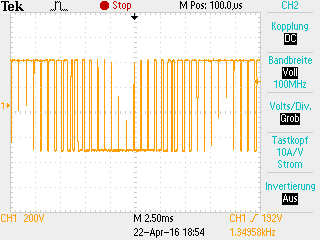
\includegraphics[width=0.48\textwidth]
  {pic/6_2_weitere_pulsmuster/6_2_1_stromform/carrier_fein/ALL0000/F0000TEK.png}
  \caption{$U_A (Orange)$}
  \label{fig:6_2_5_0}
  \end{center}
\end{figure}


\begin{figure}[H]
  \begin{center}
  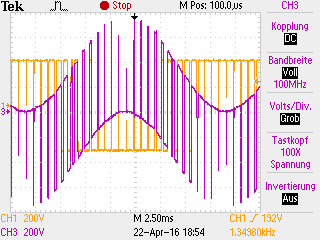
\includegraphics[width=0.48\textwidth]
  {pic/6_2_weitere_pulsmuster/6_2_1_stromform/carrier_fein/ALL0001/F0001TEK.png}
  \caption{$U_A (Orange), U_L (Violett)$}
  \label{fig:6_2_5_1}
  \end{center}
\end{figure}


\begin{figure}[H]
  \begin{center}
  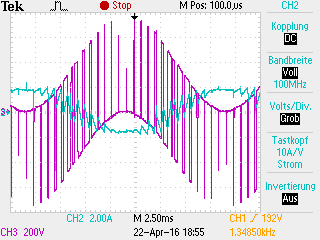
\includegraphics[width=0.48\textwidth]
  {pic/6_2_weitere_pulsmuster/6_2_1_stromform/carrier_fein/ALL0002/F0002TEK.png}
  \caption{$U_L (Violett), I_{L1} (Hellblau)$}
  \label{fig:6_2_5_2}
  \end{center}
\end{figure}



\textbf{Wirk und Blindleistung}\\

\begin{figure}[H]
  \begin{center}
  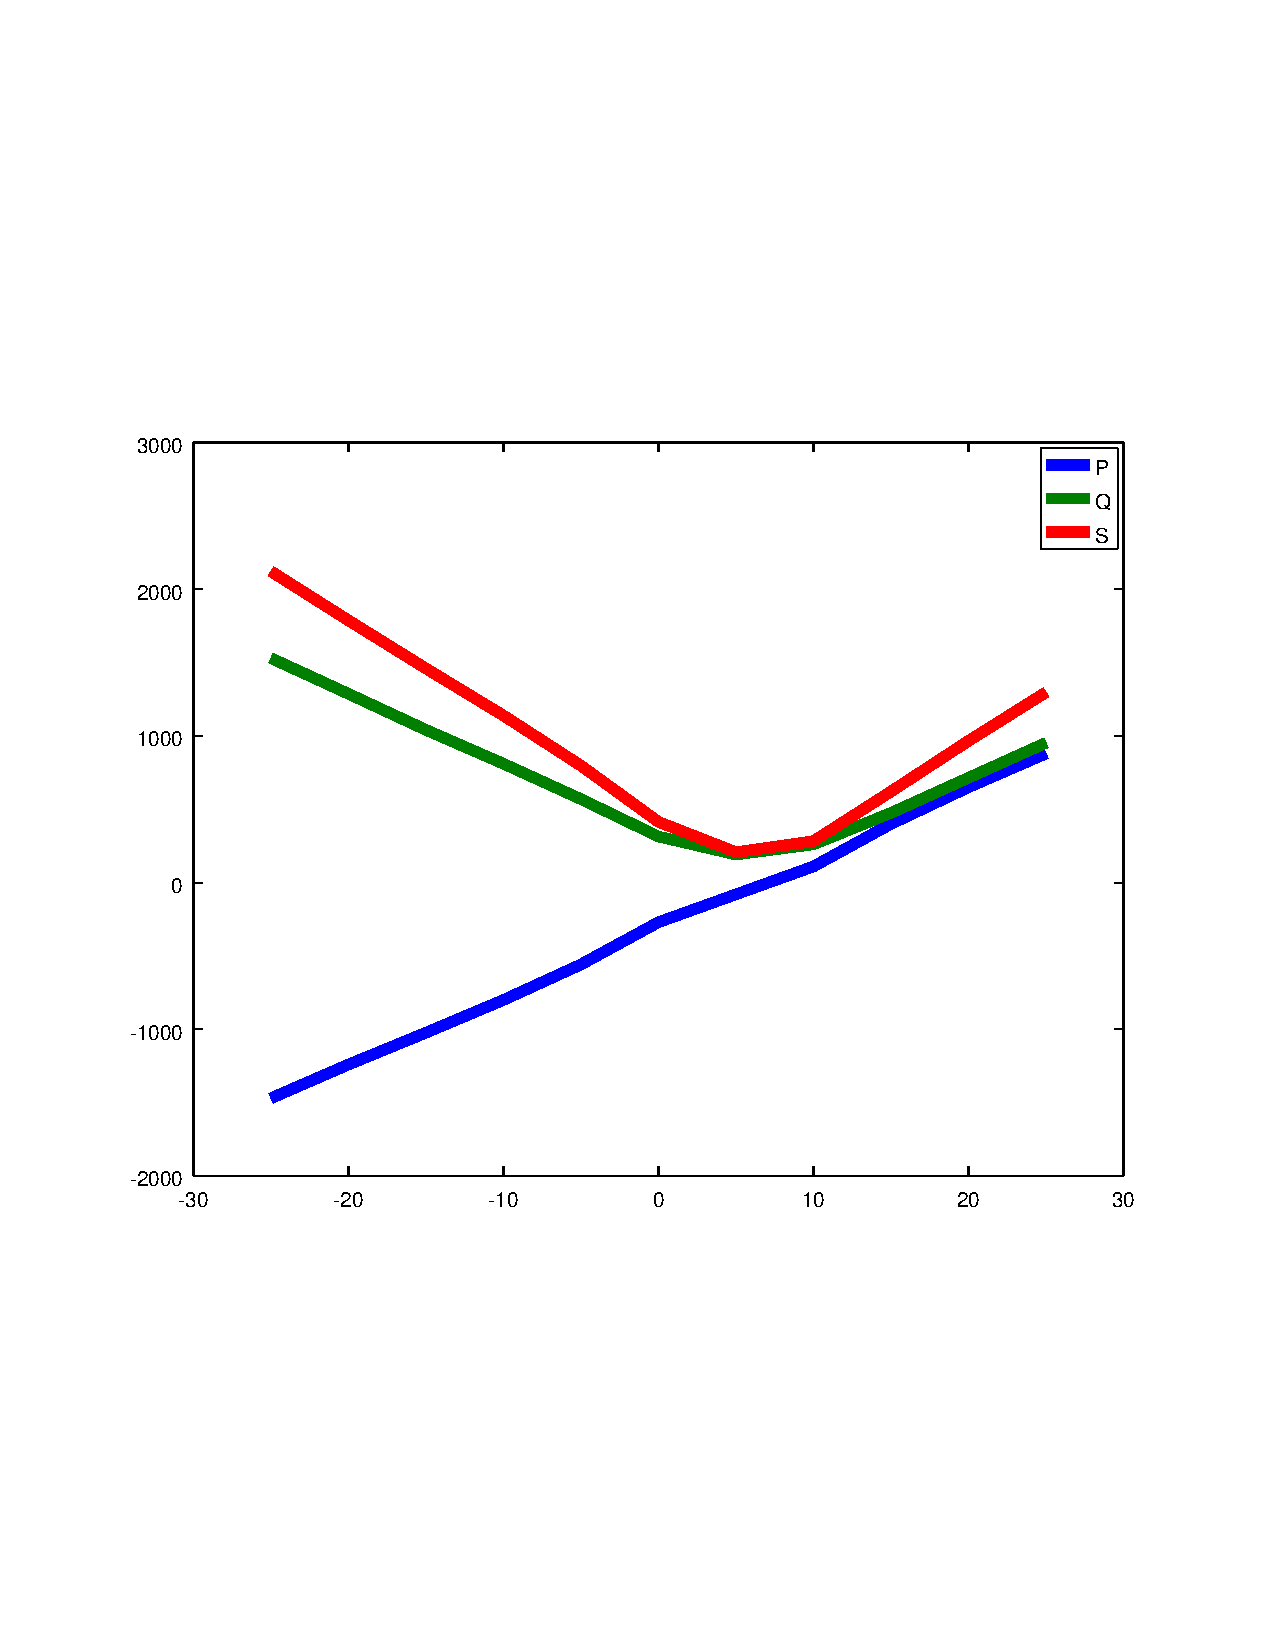
\includegraphics[width=0.5\textwidth, trim={1cm 6.5cm 2cm 7cm},clip]{pic/6_2_weitere_pulsmuster/6_2_2_einst_wirk_und_blindleistung/Sinus_fein_6_2_2_alpha.pdf}
  \caption{$P(\theta), Q(\theta), S(\theta)$}
  \label{fig:6_1_5_3}
  \end{center}
\end{figure}


\begin{figure}[H]
  \begin{center}
  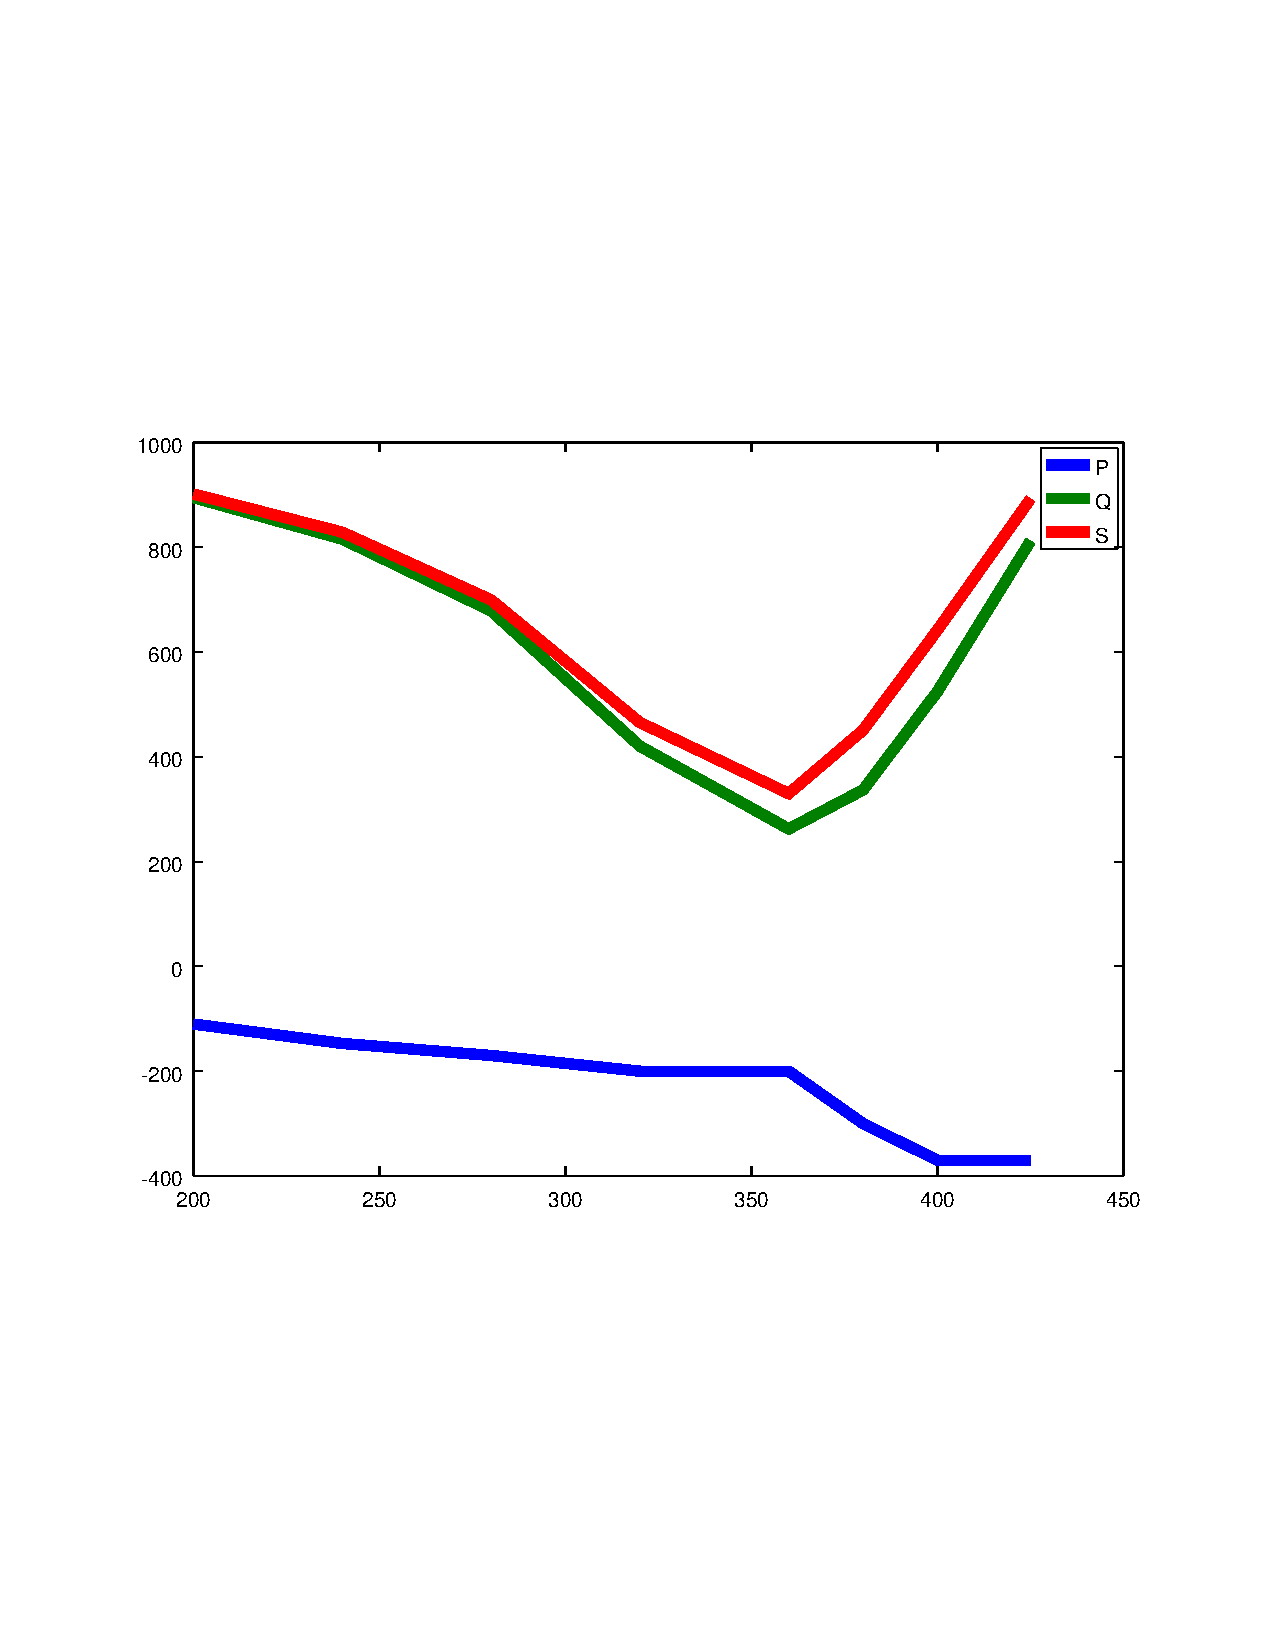
\includegraphics[width=0.5\textwidth, trim={1cm 6.5cm 2cm 7cm},clip]{pic/6_2_weitere_pulsmuster/6_2_2_einst_wirk_und_blindleistung/Sinus_fein_6_2_2_udc.pdf}
  \caption{$P(U_{dc}), Q(U_{dc}), S(U_{dc})$}
  \label{fig:6_1_5_4}
  \end{center}
\end{figure}

